\documentclass{article}
\usepackage{pgfplots}
\title{KEEL: ROC output}
\begin{document}
\maketitle
\hfill \break
File: TEST
\hfill \break
\hfill \break
\begin{tikzpicture}
\begin{axis} [xlabel=False positive rate,
ylabel=True positive rate,axis x line=bottom,
axis y line=left]
\addplot coordinates { (0,0)(0,1)(1,1)};\end{axis}
\end{tikzpicture}\hfill \break
 AUC:1.0
\hfill \break
\hfill \break
File: TRAINING
\hfill \break
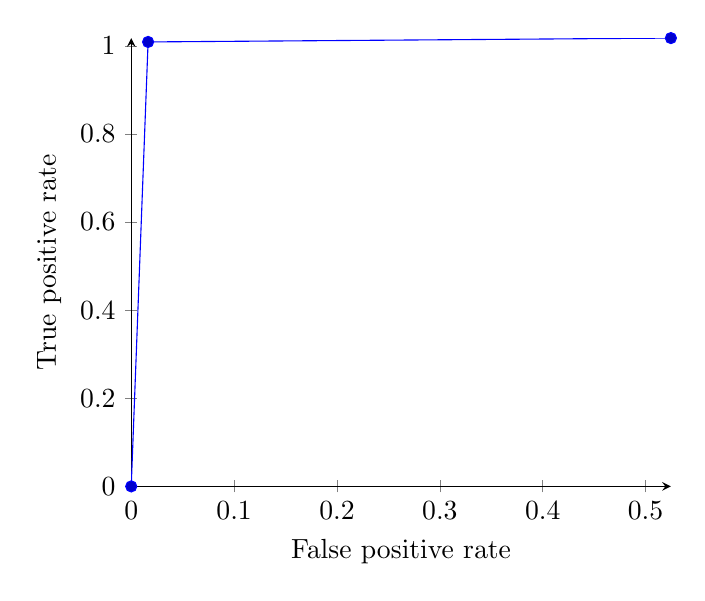
\begin{tikzpicture}
\begin{axis} [xlabel=False positive rate,
ylabel=True positive rate,axis x line=bottom,
axis y line=left]
\addplot coordinates { (0,0)(0.01639344262295082,1.0087719298245637)(0.5245901639344265,1.017543859649125) };\end{axis}
\end{tikzpicture}\hfill \break
 AUC:0.5231521426517127
\hfill \break
\end{document}